\documentclass[11pt,letterpaper]{article}
\usepackage[margin=0.87in]{geometry}
\usepackage[T1]{fontenc}
\usepackage{lmodern}
\usepackage{microtype}
\usepackage{amsmath}
\usepackage{xcolor}
\usepackage{graphicx}
\usepackage{tikz}
\usepackage{pgfplots}
\pgfplotsset{compat=1.18}
\usetikzlibrary{arrows.meta,calc,positioning,patterns,decorations.pathmorphing,shapes.misc}
\usepackage{booktabs,tabularx,array}
\usepackage{float}
\usepackage{needspace}
\usepackage[font=small,labelfont=bf,labelsep=period,skip=4pt]{caption}
\usepackage{fancyhdr}
\usepackage[colorlinks=true,linkcolor=teal!65!black,urlcolor=teal!65!black,citecolor=teal!65!black]{hyperref}

% Palette (as in the plain-language edition of paper 1)
\definecolor{ink}{HTML}{17324D}
\definecolor{accent}{HTML}{176B70}
\definecolor{pale}{HTML}{EDF5F4}
\definecolor{curl}{HTML}{C8742B}     % the curled arrangement
\definecolor{curlpale}{HTML}{F6E3D3}
\definecolor{flat}{HTML}{2E7D8C}     % the flat arrangement
\definecolor{flatpale}{HTML}{D6ECF0}
\definecolor{melt}{HTML}{8E6C8A}     % the random tangle, and the knot
\definecolor{meltpale}{HTML}{E9DEE8}
\definecolor{sun}{HTML}{E0A526}
\definecolor{no}{HTML}{B03A2E}
\definecolor{kExact}{HTML}{176B70}
\definecolor{kMeas}{HTML}{2F5F9E}
\definecolor{kPub}{HTML}{5A5A5A}
\definecolor{kOurs}{HTML}{9A5B00}
\definecolor{kClaim}{HTML}{8A2D5A}

\setlength{\parindent}{0pt}
\setlength{\parskip}{0.62em}
\renewcommand{\baselinestretch}{1.08}
\setlength{\headheight}{14pt}
\pagestyle{fancy}
\fancyhf{}
\fancyhead[L]{\small\color{ink}Two ways to read a space}
\fancyhead[R]{\small Plain-language edition}
\fancyfoot[C]{\small\thepage}
\renewcommand{\headrulewidth}{0.3pt}
\hypersetup{pdftitle={Two ways to read a space: the story behind the calculation},pdfauthor={Emily Smith}}

% Chapter opener, sub-heading, take-away box
\newcommand{\chapterpage}[2]{\par\Needspace{16\baselineskip}\vspace{1.4em}{\color{accent}\small\textbf{#1}}\par\vspace{0.2em}{\color{ink}\LARGE\bfseries #2}\par\vspace{0.5em}}
\newcommand{\takeaway}[1]{\par\medskip\noindent\colorbox{pale}{\parbox{\dimexpr\linewidth-2\fboxsep\relax}{\vspace{0.35em}\textbf{The point to keep:} #1\vspace{0.35em}}}\par\medskip}
\newcommand{\whyhere}[1]{\par\medskip\noindent{\color{accent}\small\textbf{Why we went here.}} {\small #1}\par\medskip}
\newcommand{\sub}[1]{\par\medskip{\color{ink}\large\bfseries #1}\par}

% Kinds of statement (project rule 10), as small tags
\newcommand{\tagbox}[2]{{\sffamily\scriptsize\colorbox{#1}{\textcolor{white}{\strut #2}}}}
\newcommand{\Exact}{\tagbox{kExact}{EXACT}}
\newcommand{\Meas}{\tagbox{kMeas}{MEASURED}}
\newcommand{\MeasX}{\tagbox{kMeas}{MEASURED, EXPLORATORY}}
\newcommand{\Pub}{\tagbox{kPub}{PUBLISHED}}
\newcommand{\Ours}{\tagbox{kOurs}{OUR READING, UNVERIFIED}}
\newcommand{\Claim}{\tagbox{kClaim}{THE AUTHOR'S CLAIM}}
\newcommand{\Sketch}{\tagbox{kPub}{SKETCH, NOT DATA}}

% A black dot and a white dot (the two kinds)
\newcommand{\bdot}[2]{\fill[ink] (#1,#2) circle (0.11);}
\newcommand{\wdot}[2]{\filldraw[fill=white,draw=ink,thick] (#1,#2) circle (0.1);}

\begin{document}
\thispagestyle{empty}
{\color{accent}\small\textbf{THE STORY BEHIND THE CALCULATION}}\par
\vspace{1em}
{\color{ink}\fontsize{29}{33}\selectfont\bfseries Two ways to read a space}\par
\vspace{0.5em}
{\raggedright\Large A map drawn from shared quantum information,\\pointed at a small model world\par}
\vspace{0.7em}
\textbf{Emily Smith}\quad Independent researcher\par
2 November 2026 \enspace\textbullet\enspace Plain-language edition of the technical draft of the same date~\cite{tech}
\vspace{0.9em}

There is more than one published way to get space out of something that is not space. This paper
takes two of them and asks a plain question: when they look at the same shapes, do they see the same
space?

\begin{figure}[H]
\centering
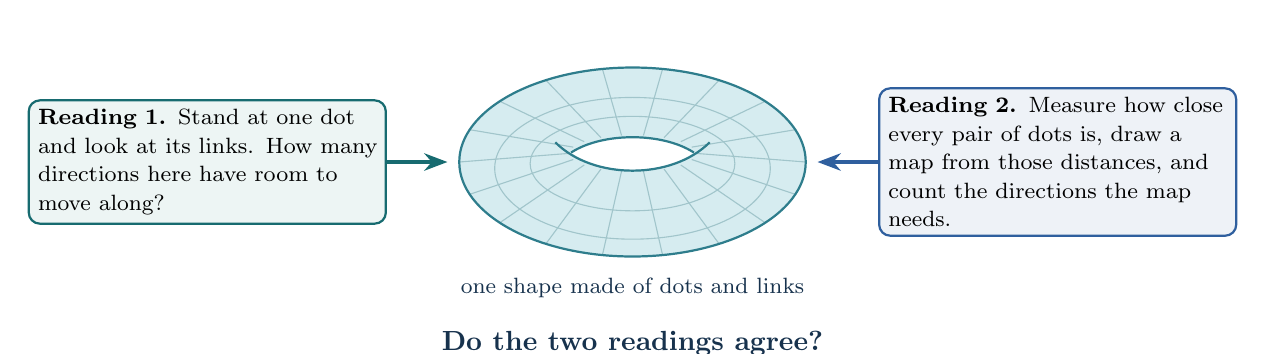
\begin{tikzpicture}[x=1cm,y=1cm,font=\small,>=Stealth]
% the shape in the middle: a doughnut of dots and links
\begin{scope}[shift={(7.6,1.2)}]
 \fill[flatpale] (0,0) ellipse (2.2 and 1.2);
 \draw[flat!45] (0,-0.08) ellipse (1.75 and 0.9);
 \draw[flat!45] (0,-0.02) ellipse (1.3 and 0.6);
 \foreach \a in {0,20,...,340} {\draw[flat!45] ({0.8*cos(\a)},{0.11+0.23*sin(\a)}) -- ({2.2*cos(\a)},{1.2*sin(\a)});}
 \fill[white] (-0.78,0.12) .. controls (-0.38,-0.17) and (0.38,-0.17) .. (0.78,0.12) .. controls (0.38,0.38) and (-0.38,0.38) .. (-0.78,0.12) -- cycle;
 \draw[flat,thick] (-0.98,0.25) .. controls (-0.5,-0.23) and (0.5,-0.23) .. (0.98,0.25);
 \draw[flat,thick] (-0.78,0.12) .. controls (-0.38,0.38) and (0.38,0.38) .. (0.78,0.12);
 \draw[flat,thick] (0,0) ellipse (2.2 and 1.2);
 \node[text=ink,align=center,font=\footnotesize] at (0,-1.6) {one shape made of dots and links};
\end{scope}
% reading 1
\node[draw=accent,thick,rounded corners=4pt,fill=pale,text width=4.3cm,align=left,font=\footnotesize] (r1) at (2.2,1.2)
 {\textbf{Reading 1.} Stand at one dot and look at its links. How many directions here have room to move along?};
% reading 2
\node[draw=kMeas,thick,rounded corners=4pt,fill=kMeas!8,text width=4.3cm,align=left,font=\footnotesize] (r2) at (13.0,1.2)
 {\textbf{Reading 2.} Measure how close every pair of dots is, draw a map from those distances, and count the directions the map needs.};
\draw[->,very thick,accent] (r1.east) -- (5.25,1.2);
\draw[->,very thick,kMeas] (r2.west) -- (9.95,1.2);
\node[text=ink,font=\normalsize\bfseries] at (7.6,-1.1) {Do the two readings agree?};
\end{tikzpicture}
\caption{The question in one picture. \Sketch\ Reading 1 belongs to the small model world this project
studies; Reading 2 is a published method from quantum physics. Chapters~2 and~3 explain each, and
Chapter~6 compares them.}
\label{fig:cover}
\end{figure}

\sub{Who is saying what}
The project keeps four kinds of statement apart, and this edition tags them where it matters, so
that a sentence is never quietly promoted from one kind to another.
\begin{itemize}\setlength{\itemsep}{1pt}
\item \Exact\ Arithmetic, or a complete listing of every possibility: true whatever a run does.
\item \Meas\ A computation whose rules and predictions were written down before it ran, with its
verdict. \MeasX\ means a computation that was not written down first, or a closer look at results
already read.
\item \Ours\ A reading of a result, offered by the author and her AI assistants and checked by no
physicist.
\item \Claim\ The author's hypothesis about reality, stated as hers.
\item \Pub\ Other researchers' published results.
\end{itemize}
Numbers in square brackets point to the sources listed at the end.

\chapterpage{1 \enspace THE PLACE WE START}{Where does space come from, and how would we know it when we saw it?}

\textbf{The author.} Emily Smith is a software engineer, not a physicist, and also a startup founder
and a foster mom. Her recreational time is limited and the computing bills are her own. Fittingly, the
project repository is called RecreationalPhysics. She works, on the side, to map her intuition about how
reality is organized onto what humanity knows about the universe, and to share what she learns with
other curious people.

\textbf{Her hypothesis.} \Claim\ Space is one settled arrangement of something deeper, which she
calls X because nobody knows what it is. X is a specific arrangement, curled up tight, and the space
we live in arose when it opened, releasing a definite amount of energy. So for her it matters whether
a curled direction counts as a direction at all, and to whom.

\textbf{The approach.} Nothing in a computer can prove a hypothesis about reality. What a computer can
do is take a small world whose rules are written out in full, in which space is an arrangement and not
a given, and ask precise questions of it. The project's first paper~\cite{paper1} did that with one
such world. This one borrows a tool from a different corner of physics, a way of reading space out of
quantum information, and points it at that world's shapes. The calculation, and what it was expected
to show, were written down before it ran, with one size held back to test the predictions.

\textbf{The parts of this paper.} Chapter~2 introduces the two published ideas that meet here.
Chapter~3 explains the borrowed tool. Chapter~4 states the question and the one choice needed to ask
it. Chapter~5 says how the shapes were read, Chapter~6 what was found, Chapter~7 what it means, and
Chapter~8 what is next, including the questions this raises for the tool's authors.

\textbf{A toy.} Physicists call a small world of that kind a \textbf{toy model}: simple enough that
every consequence of its rules can be counted or simulated, and not to be mistaken for the real thing.
Ours is \textbf{the toy} from here on.

\chapterpage{2 \enspace TWO PUBLISHED IDEAS}{A network that curves, and space read from quantum information}

\sub{The first idea: a network whose energy is curvature}
\Pub\ Carlo Trugenberger, Christy Kelly and Fabio Biancalana built a model of space with no space in
it~\cite{T25,KTB19}: only \textbf{dots} and \textbf{links}, with no positions. A dot has no place, only
neighbors. The dots come in two kinds, black and white, and a link always joins a black dot to a white
one. Every dot has exactly four links, and no two dots share more than two neighbors. Four links that
close a loop make a \textbf{square}. The list of which dots are linked to which is the network's \textbf{wiring}.

\Pub\ The energy is counted link by link from squares: a link that borders exactly two squares is free,
a missing square costs 16 units, and a third square on a link costs 4. With those prices the energy is
a network version of the curvature in Einstein's theory of gravity. This is \textbf{the published
model}. The toy keeps all of it and turns one price into a knob: a third square costs $4\lambda$, where
$\lambda$ (lambda) can be turned up or down. Only $\lambda = 1$ is the published model.

\begin{figure}[H]
\centering
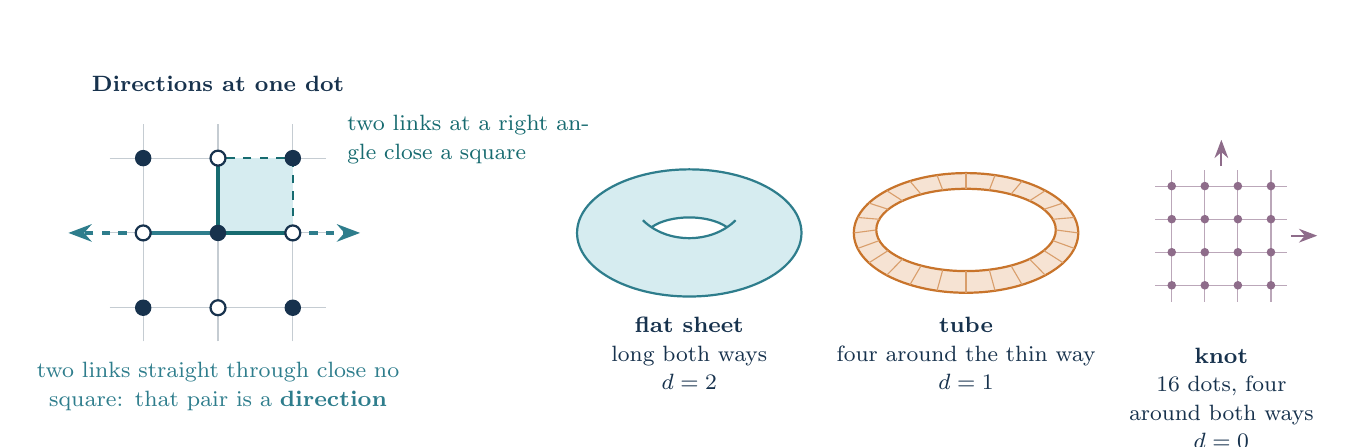
\begin{tikzpicture}[x=0.95cm,y=0.95cm,font=\footnotesize,>=Stealth]
% ---------- left: directions at a dot
\begin{scope}
 \foreach \i in {0,1,2} {\draw[ink!25] (\i,-0.45) -- (\i,2.45); \draw[ink!25] (-0.45,\i) -- (2.45,\i);}
 \fill[flatpale] (1,1) rectangle (2,2);
 \draw[very thick,accent] (2,1) -- (1,1) -- (1,2);
 \draw[thick,accent,dashed] (2,1) -- (2,2) -- (1,2);
 \draw[very thick,flat] (0,1) -- (1,1);
 \draw[very thick,flat,dashed,->] (0,1) -- (-1.0,1);
 \draw[very thick,flat,dashed,->] (2,1) -- (2.9,1);
 \foreach \i in {0,1,2} \foreach \j in {0,1,2} {
  \pgfmathtruncatemacro{\p}{mod(\i+\j,2)}
  \ifnum\p=0 \bdot{\i}{\j} \else \wdot{\i}{\j} \fi}
 \node[font=\footnotesize\bfseries,text=ink] at (1,3.0) {Directions at one dot};
 \node[text=accent,anchor=west,align=left,text width=3.2cm] at (2.6,2.25) {two links at a right angle close a square};
 \node[text=flat,anchor=north,align=center,text width=4.6cm] at (1,-0.6) {two links straight through close no square: that pair is a \textbf{direction}};
\end{scope}
% ---------- right: the three shapes
\begin{scope}[shift={(7.3,1.0)}]
 % flat sheet: a fat doughnut
 \fill[flatpale] (0,0) ellipse (1.5 and 0.85);
 \fill[white] (-0.5,0.08) .. controls (-0.25,-0.1) and (0.25,-0.1) .. (0.5,0.08) .. controls (0.25,0.25) and (-0.25,0.25) .. (-0.5,0.08) -- cycle;
 \draw[flat,thick] (-0.62,0.17) .. controls (-0.3,-0.15) and (0.3,-0.15) .. (0.62,0.17);
 \draw[flat,thick] (-0.5,0.08) .. controls (-0.25,0.25) and (0.25,0.25) .. (0.5,0.08);
 \draw[flat,thick] (0,0) ellipse (1.5 and 0.85);
 \node[text=ink,align=center,anchor=north] at (0,-1.0) {\textbf{flat sheet}\\long both ways\\$d=2$};
\end{scope}
\begin{scope}[shift={(11.0,1.0)}]
 % tube: a thin ring
 \fill[curlpale,even odd rule] (0,0) ellipse (1.5 and 0.8) (0,0.04) ellipse (1.2 and 0.55);
 \draw[curl,thick] (0,0) ellipse (1.5 and 0.8);
 \draw[curl,thick] (0,0.04) ellipse (1.2 and 0.55);
 \foreach \a in {0,15,...,345} {\draw[curl!70] ({1.2*cos(\a)},{0.04+0.55*sin(\a)}) -- ({1.5*cos(\a)},{0.8*sin(\a)});}
 \node[text=ink,align=center,anchor=north] at (0,-1.0) {\textbf{tube}\\four around the thin way\\$d=1$};
\end{scope}
\begin{scope}[shift={(13.75,0.3)},x=0.42cm,y=0.42cm]
 % knot: a 4 by 4 grid that wraps both ways
 \foreach \i in {0,...,3} {\draw[melt!60] (\i,-0.5) -- (\i,3.5); \draw[melt!60] (-0.5,\i) -- (3.5,\i);}
 \foreach \i in {0,...,3} \foreach \j in {0,...,3} {\fill[melt] (\i,\j) circle (0.13);}
 \draw[->,melt,thick] (3.6,1.5) -- (4.4,1.5); \draw[->,melt,thick] (1.5,3.6) -- (1.5,4.4);
 \node[text=ink,align=center,anchor=north] at (1.5,-1.6) {\textbf{knot}\\16 dots, four\\around both ways\\$d=0$};
\end{scope}
\end{tikzpicture}
\caption{The toy's two ingredients for this paper. \Exact\ Left: at a dot, four links make six pairs;
a pair at a right angle closes a square, and a pair that runs straight through closes none. The
\textbf{toy's count} $d$ is the number of pairs that close no square. Right: three shapes, each a grid
whose edges are joined both ways round, so none has an end. The sheet is a fat doughnut, long both
ways. The tube is a thin ring: its thin way round is only four steps, so walking round it is itself a
square, and that direction no longer counts. The knot is curled both ways. (The doughnut and ring are
drawn bent; the network itself has no positions and is bent nowhere.)}
\label{fig:toy}
\end{figure}

Two words are kept apart from here on. \textbf{Flat} is about each dot's surroundings: every link on
exactly two squares, the wiring of a plain grid, at zero energy. \textbf{Wide} is about the whole shape:
how many steps it takes to walk round it and come back. The sheet is flat and wide; the tube is neither.

\Exact\ With the knob above 1, the tube sits $4(\lambda-1)$ units per dot above the flat sheet, and gives
that much off if it opens. The author calls that release \textbf{the burp}. \Meas\ Paper~1~\cite{paper1}
watched tubes open at $\lambda = 1.25$. What they opened into was flat at every dot but still narrow:
a ring whose shortest way round is six steps instead of four. This paper reads some of those rings.

\textbf{Her positions on the toy.} \Claim\ The author holds that, taken as a whole, no network she uses
has $\lambda$ above 1: it is 1 or below everywhere, the curled X looked at one part at a time being the
exception. She holds that the black dots and the white dots are two distinct kinds, and that within a
kind every dot is the same. And she holds that the dots belong to the two-dimensional picture only: the
deeper ingredients are twist and curl. None of this is assumed below.

\sub{The second idea: space read from quantum information}
\Pub\ ChunJun Cao, Sean Carroll and Spyridon Michalakis start somewhere else entirely~\cite{CCM16,CC17}.
In quantum physics, everything that can be known about a system is packed into one object, its
\textbf{state}. Split a system into parts, and the parts of a state can be tied together so that
learning about one tells you something about another, with nothing in between: that tie is
\textbf{entanglement}. Their idea is to begin with a quantum state and no space at all, measure how
strongly each pair of parts is tied, and read a geometry off those ties. Their recipe for the reading is
called \textbf{the reader} here. They say plainly that they
assume no energy rule, and that the split into parts is taken as given~\cite{CCM16}. Their second paper
goes on toward Einstein's equation~\cite{CC17}.

The two ideas meet at one point. Each ends with a list of which things are close to which, and each
asks what space that list describes.

\takeaway{The toy is a network of black and white dots whose energy is a curvature; it counts the
directions at a dot, $d$: two on the flat sheet, one on the tube, none on the knot. Carroll and his
colleagues read space from how strongly the parts of a quantum state are tied. This paper hands the
toy's shapes to their reader.}

\chapterpage{3 \enspace THE TOOL}{How do you draw a map from a table of shared information?}

The reader works in four steps (Figure~\ref{fig:reader}).

\textbf{Step 1: shared information.} \Pub\ The strength of the tie between two parts is measured as
\textbf{shared information}: how much knowing one part tells you about the other, counted in bits. Two
coins that always land the same way share one bit: see one and you know the other. Two unrelated coins
share none. Physicists call it mutual information.

\textbf{Step 2: sharing becomes distance.} \Pub\ The more two parts share, the closer they are put. Each
pair that shares anything gets a direct line whose length is set by how much it shares, and a pair that
shares nothing gets no direct line. In their examples the length is minus the natural logarithm of the
share, measured against the most two parts can share:

\begin{center}
\renewcommand{\arraystretch}{1.15}
\begin{tabular}{lcccc}
\toprule
Share, as a fraction of the most possible & all of it & a half & a tenth & a thousandth \\
Length of the direct line & 0 & 0.69 & 2.3 & 6.9 \\
\bottomrule
\end{tabular}
\end{center}

The distance between any two parts is then the shortest chain of direct lines between them.

\textbf{Step 3: a table of distances becomes a map.} \Pub\ The back of an old road atlas has a mileage
chart: the driving distance between every pair of cities, and nothing else. From that chart alone you
could redraw the map, putting each city where its distances to all the others fit best. The reader does
exactly this with the parts. The standard recipe is called multidimensional scaling.

\textbf{Step 4: count the directions.} \Pub\ A mileage chart for cities on flat ground fits a flat page
perfectly: two directions, north and south, east and west, and nothing left over. The recipe reports how
much of the map's \textbf{spread} lies along each of its directions, largest first; for cities on flat
ground, two directions carry all of it. When the distances do not fit any page exactly, a third and
fourth direction carry some spread too, and someone has to decide how much counts. Their papers leave
that open; their own examples call a chain of 100 quantum parts one-dimensional and a patch of a known
two-dimensional quantum system two-dimensional~\cite{CCM16}. For this paper the rule was fixed before
any calculation: a direction counts if its spread is at least a tenth of the largest. The tenth is a
choice, not a law. The number of directions that pass is \textbf{the reader's count}.

\begin{figure}[H]
\centering
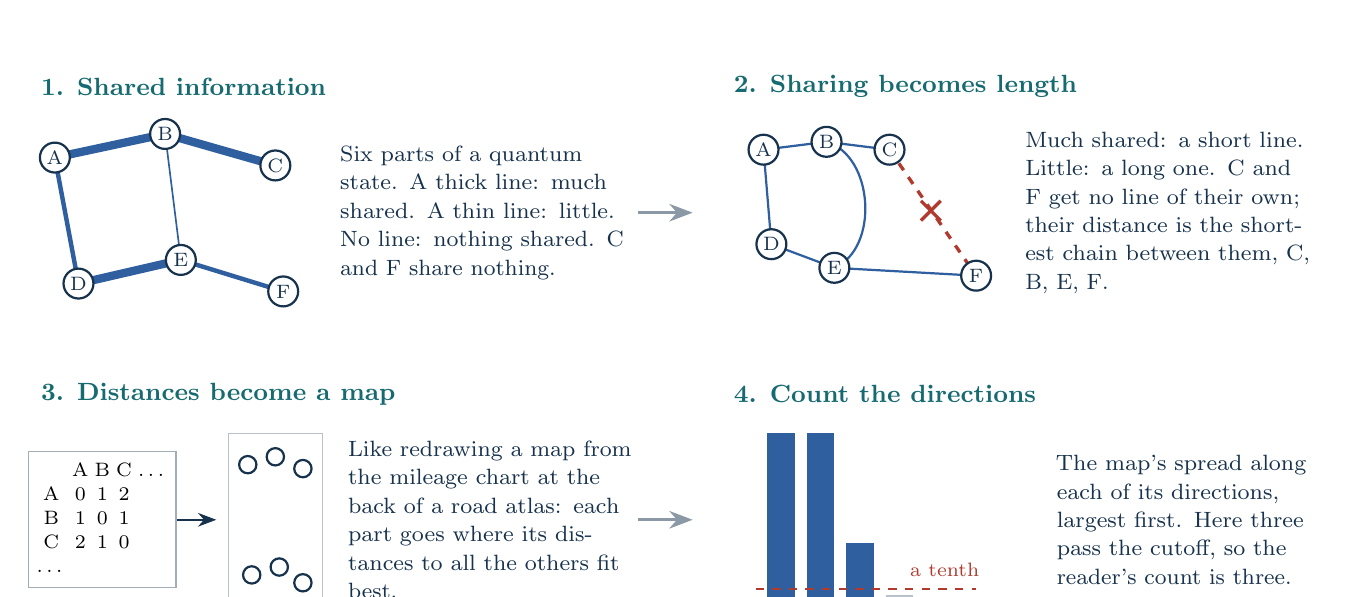
\begin{tikzpicture}[x=1cm,y=1cm,font=\footnotesize,>=Stealth]
% ---------- 1. shared information
\begin{scope}
 \node[font=\small\bfseries,text=accent,anchor=west] at (-0.3,2.9) {1. Shared information};
 \coordinate (A) at (0,2); \coordinate (B) at (1.4,2.3); \coordinate (C) at (2.8,1.9);
 \coordinate (D) at (0.3,0.4); \coordinate (E) at (1.6,0.7); \coordinate (F) at (2.9,0.3);
 \draw[kMeas,line width=3pt] (A) -- (B); \draw[kMeas,line width=3pt] (B) -- (C);
 \draw[kMeas,line width=3pt] (D) -- (E); \draw[kMeas,line width=1.6pt] (E) -- (F);
 \draw[kMeas,line width=1.6pt] (A) -- (D); \draw[kMeas,line width=0.6pt] (B) -- (E);
 \foreach \p/\n in {A/A,B/B,C/C,D/D,E/E,F/F} {\filldraw[fill=white,draw=ink,thick] (\p) circle (0.19); \node[font=\scriptsize,text=ink] at (\p) {\n};}
 \node[text=ink,align=left,text width=3.6cm,anchor=west] at (3.5,1.3) {Six parts of a quantum state. A thick line: much shared. A thin line: little. No line: nothing shared. C and F share nothing.};
\end{scope}
\draw[->,very thick,ink!50] (7.4,1.3) -- (8.1,1.3);
% ---------- 2. lengths
\begin{scope}[shift={(8.8,0)}]
 \node[font=\small\bfseries,text=accent,anchor=west] at (-0.3,2.9) {2. Sharing becomes length};
 \coordinate (A) at (0.2,2.1); \coordinate (B) at (1.0,2.2); \coordinate (C) at (1.8,2.1);
 \coordinate (D) at (0.3,0.9); \coordinate (E) at (1.1,0.6); \coordinate (F) at (2.9,0.5);
 \draw[kMeas,thick] (A) -- (B) -- (C); \draw[kMeas,thick] (D) -- (E) -- (F); \draw[kMeas,thick] (A) -- (D);
 \draw[kMeas,thick] (B) to[bend left=70] (E);
 \draw[no,very thick,dashed] (C) -- (F);
 \draw[no,very thick] (2.2,1.2) -- (2.45,1.45) (2.2,1.45) -- (2.45,1.2);
 \foreach \p/\n in {A/A,B/B,C/C,D/D,E/E,F/F} {\filldraw[fill=white,draw=ink,thick] (\p) circle (0.19); \node[font=\scriptsize,text=ink] at (\p) {\n};}
 \node[text=ink,align=left,text width=3.7cm,anchor=west] at (3.4,1.3) {Much shared: a short line. Little: a long one. C and F get no line of their own; their distance is the shortest chain between them, C, B, E, F.};
\end{scope}
% ---------- 3. map
\begin{scope}[shift={(0,-3.9)}]
 \node[font=\small\bfseries,text=accent,anchor=west] at (-0.3,2.9) {3. Distances become a map};
 \node[draw=ink!40,fill=white,font=\scriptsize,align=center,inner sep=3pt] at (0.6,1.3) {\renewcommand{\arraystretch}{1.0}\begin{tabular}{@{}c@{\;}c@{\;}c@{\;}c@{\;}c@{}}&A&B&C&\ldots\\A&0&1&2&\\B&1&0&1&\\C&2&1&0&\\\ldots&&&&\end{tabular}};
 \draw[->,thick,ink] (1.55,1.3) -- (2.05,1.3);
 \draw[ink!30] (2.2,0.2) rectangle (3.4,2.4);
 \foreach \p in {(2.45,2.0),(2.8,2.1),(3.15,1.95),(2.5,0.6),(2.85,0.7),(3.15,0.5)} {\filldraw[fill=white,draw=ink,thick] \p circle (0.11);}
 \node[text=ink,align=left,text width=3.6cm,anchor=west] at (3.6,1.3) {Like redrawing a map from the mileage chart at the back of a road atlas: each part goes where its distances to all the others fit best.};
\end{scope}
\draw[->,very thick,ink!50] (7.4,-2.6) -- (8.1,-2.6);
% ---------- 4. count
\begin{scope}[shift={(8.8,-3.9)}]
 \node[font=\small\bfseries,text=accent,anchor=west] at (-0.3,2.9) {4. Count the directions};
 \foreach \h/\c [count=\k] in {2.2/kMeas,2.2/kMeas,0.8/kMeas,0.15/ink!30,0.08/ink!30} {\fill[\c] (-0.25+0.5*\k,0.2) rectangle (0.1+0.5*\k,0.2+\h);}
 \draw[ink] (0.1,0.2) -- (2.9,0.2);
 \draw[no,thick,dashed] (0.1,0.42) -- (2.9,0.42);
 \node[text=no,anchor=south,font=\scriptsize] at (2.5,0.45) {a tenth};
 \node[text=ink,align=left,text width=3.4cm,anchor=west] at (3.8,1.3) {The map's spread along each of its directions, largest first. Here three pass the cutoff, so the reader's count is three.};
\end{scope}
\end{tikzpicture}
\caption{Carroll's reader in four steps. \Pub\ Steps 1 to 3 are the published recipe~\cite{CCM16}.
\Sketch\ The numbers are made up for the drawing. The cutoff in step 4, a tenth of the largest spread,
was chosen for this paper before any calculation; the published papers leave it open.}
\label{fig:reader}
\end{figure}

\takeaway{Shared information becomes distance, a full table of distances becomes a map, and the number
of directions the map needs is the reader's count. Where the map does not fit a page exactly, the count
depends on a cutoff, which here is a tenth of the largest spread, fixed in advance.}

\chapterpage{4 \enspace THE QUESTION}{What does the reader see when it is handed a wiring?}

The toy has no quantum state; it has a wiring. To hand it to the reader, one choice is needed.

\sub{The one choice}
Give each dot one quantum part, and give every linked pair the same share of information, and every
unlinked pair none. The toy itself says nothing more: in it, two dots are linked or they are not, and
every link is like every other.

\Exact\ Then every direct line has the same length, and the distance between two dots is simply the
number of steps along links between them, times that length. The map's directions all scale together,
so the reader's count does not depend on how large the share is. With this choice, the reader is just
a map drawn from step counts.

\sub{Does a quantum state like that exist?}
\Pub\ One published state is built from a wiring: Marcelo Diamantini and Carlo Trugenberger turned the
link list of a network into a quantum state on two copies of its dots~\cite{DT17}. \Exact\ Computed for
this paper on an 8~by~8 flat sheet: a linked pair shares 0.0117 bits, about 33 times what every other
pair shares, 0.00036 bits. So the sharing follows the wiring.

\Exact\ But that faint share between every pair matters. Carroll's rule gives every pair that shares
anything a direct line, and a faint share still makes a line shorter than two links:

\begin{center}
\renewcommand{\arraystretch}{1.15}
\begin{tabular}{lr}
\toprule
One link (a linked pair's share) & length 5.14 \\
Two links in a row & length 10.28 \\
\textbf{A direct line between any other pair (the faint share)} & \textbf{length 8.63} \\
\bottomrule
\end{tabular}
\end{center}

So no pair is ever more than 8.63 apart, every pair looks close, and the map comes out as one direction
followed by five at about three quarters of it: no shape at all. Subtract the faint background first, and the
wiring's map returns. \Ours\ So a quantum state whose sharing follows a wiring exists, but only after a
step, subtracting the background, that Carroll's papers do not take. The state is built from the wiring,
so it checks the reader; it does not test how a geometry could arise.

\begin{center}
\colorbox{pale}{\parbox{0.86\linewidth}{\centering\vspace{0.3em}\large\bfseries\color{ink}
Given the toy's shapes, does Carroll's reader count the same directions as the toy does:\\
two on the sheet, one on the tube, none on the knot?\vspace{0.3em}}}
\end{center}

\whyhere{Her picture of the birth of space is a curled direction opening. If an independent reader,
built in quantum physics with no knowledge of the toy, did not see a curled direction as different from
an open one, the toy's count would be a convention of the toy and nothing more.}

\chapterpage{5 \enspace WHAT WE TRIED}{Why not read the whole doughnut?}

\sub{Every way round counts twice}
\Exact\ A loop cannot be laid along a line. Eight dots in a ring, each one step from the next, need a
page: placed on a circle they fit, and a circle takes two directions. So every way round that a shape
wraps takes a pair of directions on the map (Figure~\ref{fig:window}, left). The flat sheet wraps two
ways, so whole it reads four; the tube wraps two ways, so it reads four; the knot reads four. Read
whole, every doughnut looks much the same: four directions each.

\sub{Windows}
So the reader is given a \textbf{window} instead: one dot, the center, and every dot within $R$ steps of
it, with their distances taken through the whole network. A window is what someone living at the center
could reach on foot within $R$ steps. Its width is $2R+1$ dots across. Windows were read at $R = 2$, 3, 4
and~6; the widest, $R = 10$, was held back, and computed only after a prediction for it had been
written from the smaller ones.

\begin{figure}[H]
\centering
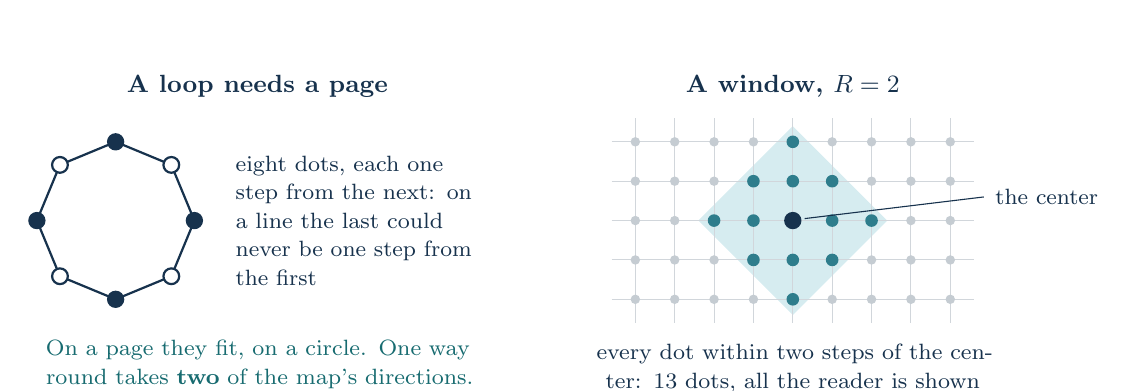
\begin{tikzpicture}[x=1cm,y=1cm,font=\footnotesize,>=Stealth]
% ---------- left: a ring of eight dots needs two directions
\begin{scope}
 \node[font=\small\bfseries,text=ink] at (1.8,3.1) {A loop needs a page};
 \foreach \k in {0,...,7} {\draw[ink,thick] ({1.0*cos(45*\k)},{1.4+1.0*sin(45*\k)}) -- ({1.0*cos(45*(\k+1))},{1.4+1.0*sin(45*(\k+1))});}
 \foreach \k in {0,...,7} {\pgfmathsetmacro{\cx}{cos(45*\k)} \pgfmathsetmacro{\cy}{1.4+sin(45*\k)} \pgfmathtruncatemacro{\p}{mod(\k,2)} \ifnum\p=0 \bdot{\cx}{\cy} \else \wdot{\cx}{\cy} \fi}
 \node[text=ink,align=left,anchor=west,text width=3.0cm] at (1.4,1.4) {eight dots, each one step from the next: on a line the last could never be one step from the first};
 \node[text=accent,align=center,text width=5.6cm,anchor=north] at (1.8,0.0) {On a page they fit, on a circle. One way round takes \textbf{two} of the map's directions.};
\end{scope}
% ---------- right: a window on the sheet
\begin{scope}[shift={(8.6,1.4)},x=0.5cm,y=0.5cm]
 \node[font=\small\bfseries,text=ink] at (0,3.4) {A window, $R=2$};
 \fill[flatpale] (0,-2.4) -- (2.4,0) -- (0,2.4) -- (-2.4,0) -- cycle;
 \foreach \x in {-4,...,4} {\draw[ink!20] (\x,-2.6) -- (\x,2.6);}
 \foreach \y in {-2,...,2} {\draw[ink!20] (-4.6,\y) -- (4.6,\y);}
 \foreach \x in {-4,...,4} \foreach \y in {-2,...,2} {
   \pgfmathtruncatemacro{\r}{abs(\x)+abs(\y)}
   \ifnum\r>2 \fill[ink!25] (\x,\y) circle (0.12); \else \fill[flat] (\x,\y) circle (0.16); \fi}
 \fill[ink] (0,0) circle (0.22);
 \node[text=ink,anchor=west,align=left] at (4.9,0.6) {the center};
 \draw[ink] (4.85,0.6) -- (0.3,0.05);
 \node[text=ink,align=center,text width=6.2cm,anchor=north] at (0,-2.9) {every dot within two steps of the center: 13 dots, all the reader is shown};
\end{scope}
\end{tikzpicture}
\caption{Why whole doughnuts cannot be read, and what is read instead. \Exact\ Left: a ring cannot be
laid on a line without stretching some step, so the map spends two directions on every way round.
Right: a window is a diamond of dots around one center (Chapter~6 says why it is a diamond and not a
circle). The reader maps only those dots.}
\label{fig:window}
\end{figure}

\sub{The shapes, and what was expected}
Three shapes were built exactly: a flat sheet 32 by 32 dots, a tube 4 around and 64 along, and the
knot. Two kinds were taken from earlier runs: four rings left by the burp, each of 1,024 dots, read
from 512 centers apiece; and four \textbf{random tangles}, warm networks of the published model in which
the wiring is jumbled, 196 dots each, read from every dot. These sizes are conveniences, not special
values.

Written down before any window was computed: the knot would read four; the flat sheet two; the tube no
more than the sheet, with its curled direction too faint to count by $R = 4$; the burp's rings the same
as the sheet; the tangles four or more.

\chapterpage{6 \enspace WHAT WE FOUND}{Five shapes, read window by window}

\sub{The knot reads four}
\Exact\ At every window size the knot reads four directions, all with equal spread. The toy counts none.
That was expected, and it is a difference of definitions, not a mistake on either side: the toy counts
directions with room in them, and the reader counts how many directions a map needs. A knot has many
directions, all short.

\sub{The flat sheet reads three, sometimes four}
\Exact\ The flat sheet reads four, four, four and three directions at $R = 2$, 3, 4 and~6. Its first two
directions are equal, as a page's should be. But a third carries between about two fifths and a half of
the largest spread at every size, and a fourth sits close to the cutoff: at $R = 4$ it is 0.101 of the
largest, a hair above the tenth, which is why the count there is four and not three. \Meas\ The
prediction of two failed.

The reason is how distance is counted. In a city laid out in square blocks, a taxi cannot cut across:
three blocks east and three north is six blocks of driving, while a crow flies about four and a quarter.
Steps along a grid are taxi distances. The dots exactly three steps from the center do not form a circle
but a diamond (Figure~\ref{fig:taxi}), and no flat page holds a diamond of equal distances, so the map
reaches for extra directions.

\begin{figure}[H]
\centering
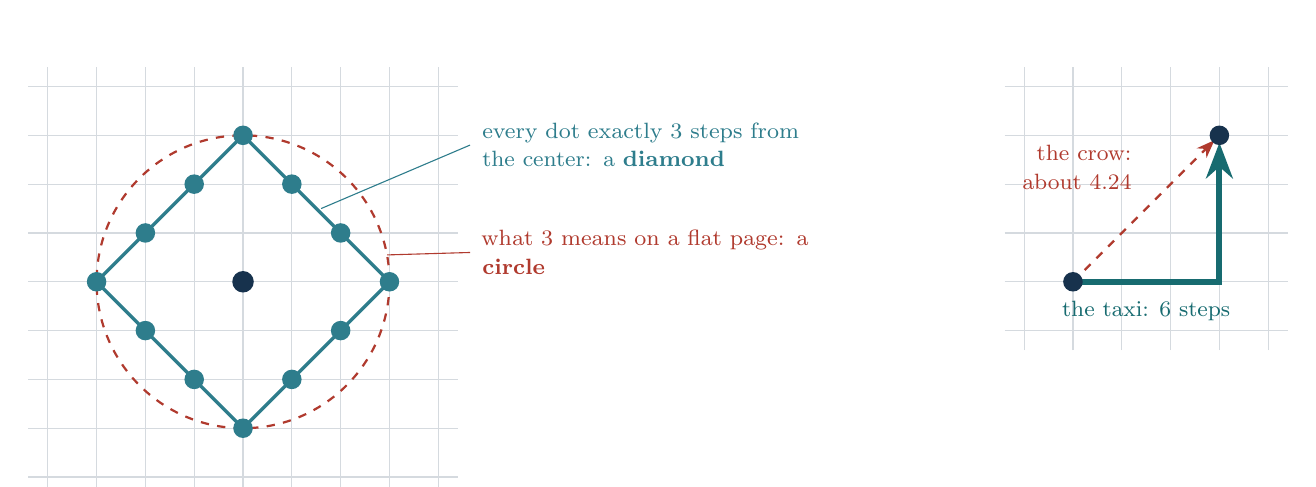
\begin{tikzpicture}[x=0.62cm,y=0.62cm,font=\footnotesize,>=Stealth]
\begin{scope}
 \foreach \x in {-4,...,4} {\draw[ink!18] (\x,-4.4) -- (\x,4.4);}
 \foreach \y in {-4,...,4} {\draw[ink!18] (-4.4,\y) -- (4.4,\y);}
 \draw[no,thick,dashed] (0,0) circle (3);
 \draw[flat,very thick] (3,0) -- (0,3) -- (-3,0) -- (0,-3) -- cycle;
 \foreach \x in {-3,...,3} \foreach \y in {-3,...,3} {
   \pgfmathtruncatemacro{\r}{abs(\x)+abs(\y)}
   \ifnum\r=3 \fill[flat] (\x,\y) circle (0.2); \fi}
 \fill[ink] (0,0) circle (0.22);
 \node[text=flat,anchor=west,align=left,text width=4.4cm] at (4.7,2.8) {every dot exactly 3 steps from the center: a \textbf{diamond}};
 \node[text=no,anchor=west,align=left,text width=4.4cm] at (4.7,0.6) {what 3 means on a flat page: a \textbf{circle}};
 \draw[flat] (4.65,2.8) -- (1.6,1.5);
 \draw[no] (4.65,0.6) -- (2.95,0.55);
\end{scope}
\begin{scope}[shift={(17,0)}]
 \foreach \x in {-1,...,4} {\draw[ink!18] (\x,-1.4) -- (\x,4.4);}
 \foreach \y in {-1,...,4} {\draw[ink!18] (-1.4,\y) -- (4.4,\y);}
 \draw[accent,line width=2.2pt,->] (0,0) -- (3,0) -- (3,2.85);
 \draw[no,thick,dashed,->] (0,0) -- (2.9,2.9);
 \fill[ink] (0,0) circle (0.2); \fill[ink] (3,3) circle (0.2);
 \node[text=accent,anchor=north] at (1.5,-0.2) {the taxi: 6 steps};
 \node[text=no,anchor=south east,align=right] at (1.4,1.7) {the crow:\\about 4.24};
\end{scope}
\end{tikzpicture}
\caption{Taxi distance is not straight-line distance. \Exact\ On a grid, steps along links are what a
taxi drives in a city of square blocks. Equal step counts make a diamond, not a circle, and the map
needs more than a page to hold it. The extra directions say more about the distance assigned to a grid
than about the toy. \Exact\ If instead the sharing between every pair fell off with straight-line
distance, the map of any patch of a flat sheet would need exactly two directions.}
\label{fig:taxi}
\end{figure}

\sub{The tube's curled direction is seen up close and fades from afar}
Think of a garden hose. An ant on it can walk round it as easily as along it; from across the yard, the
hose is a line. The tube is a hose four dots round.

\Exact\ In the tube's windows the long direction carries the largest spread, and the curled direction
shows up as a pair. Its share of the largest spread falls as the window widens: 0.61, 0.43, 0.31 and
0.20 at $R = 2$, 3, 4 and~6 (Figure~\ref{fig:fade}). \Meas\ So the ranking held: at $R = 4$ the tube read
three directions against the sheet's four. But the prediction that the curled direction would be too
faint to count by then failed: it was four times stronger than predicted.

\Meas\ From $R = 4$ and~6 alone, a rule was fitted, the share falling as the window's width to the power
$-1.24$, and written down before the widest window was computed: at $R = 10$, 0.108, with a range of
0.076 to 0.141. \textbf{The widest window measured 0.112.} The prediction held.

\begin{figure}[H]
\centering
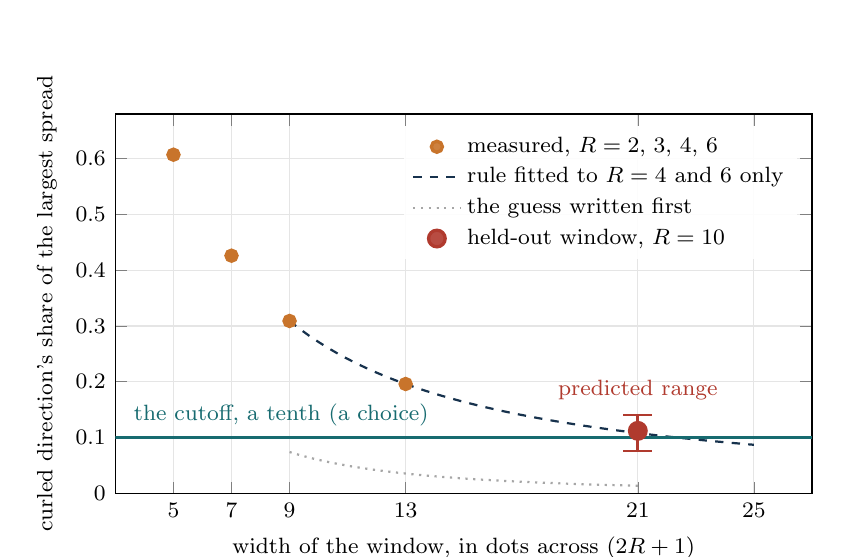
\begin{tikzpicture}
\begin{axis}[width=0.86\linewidth,height=6.4cm,xlabel={width of the window, in dots across ($2R+1$)},ylabel={curled direction's share of the largest spread},xmin=3,xmax=27,ymin=0,ymax=0.68,xtick={5,7,9,13,21,25},ytick={0,0.1,0.2,0.3,0.4,0.5,0.6},yticklabel style={/pgf/number format/fixed},grid=both,grid style={gray!20},tick label style={font=\footnotesize},label style={font=\footnotesize},legend style={at={(0.98,0.97)},anchor=north east,font=\footnotesize,draw=none,fill=white,fill opacity=0.9,text opacity=1},legend cell align=left]
\addplot[curl,very thick,mark=*,mark options={fill=curl},only marks] coordinates {(5,0.607) (7,0.426) (9,0.309) (13,0.196)};
\addlegendentry{measured, $R = 2$, 3, 4, 6}
\addplot[ink,thick,dashed,domain=9:25,samples=50] {0.309*(x/9)^(-1.24)};
\addlegendentry{rule fitted to $R = 4$ and 6 only}
\addplot[gray!70,thick,dotted,domain=9:21,samples=30] {6/x^2};
\addlegendentry{the guess written first}
\addplot[no,very thick,mark=*,mark size=3pt,mark options={fill=no},only marks] coordinates {(21,0.112)};
\addlegendentry{held-out window, $R = 10$}
\draw[no,very thick] (axis cs:21,0.076) -- (axis cs:21,0.141);
\draw[no,thick] (axis cs:20.5,0.076) -- (axis cs:21.5,0.076) (axis cs:20.5,0.141) -- (axis cs:21.5,0.141);
\node[font=\footnotesize,text=no,anchor=south] at (axis cs:21,0.15) {predicted range};
\draw[accent,thick] (axis cs:3,0.1) -- (axis cs:27,0.1);
\node[font=\footnotesize,text=accent,anchor=south west] at (axis cs:3.3,0.103) {the cutoff, a tenth (a choice)};
\end{axis}
\end{tikzpicture}
\caption{The hose seen from farther and farther away. Points at $R = 2$ to 6: \Exact. The fitted rule and
its prediction: \Meas, written down before the held-out window at $R = 10$ (width 21) was computed; the
measured 0.112 lands inside the predicted range of 0.076 to 0.141. The dotted line is the first guess,
which missed by a factor of four. Extended (not computed), the fitted rule crosses the cutoff at windows
about 22 dots across.}
\label{fig:fade}
\end{figure}

\sub{The burp's rings read one direction from afar}
\Meas\ The rings left by the burp read five, four, four and three directions at $R = 2$, 3, 4 and~6, in
nearly every one of their 512 windows. At $R = 10$ they read one, in 506 of 512. The prediction that they
would read like the flat sheet failed at the smallest window and at the largest. \Ours\ The reason is
the hose again: these rings are narrow, their shortest way round only six steps, so a wide window wraps
right round them, and from that far the reader calls them a line.

\sub{The random tangles read many}
\Meas\ The jumbled networks read four or more directions at $R = 3$ in 778 of 784 windows, and more as
the window widens, up to 17, as expected: a tangle has no shape a page can hold.

\sub{One miss that was the window's fault}
\Meas\ At $R = 10$ the flat sheet was predicted to read three and read four, its fourth direction again
right on the cutoff. \Exact\ A check made after the reading, not written down in advance, found the
cause: a window ten steps out holds pairs twenty steps apart, more than halfway round a sheet 32 dots
wide, so some of their shortest paths go round the back of the doughnut. On a sheet 64 by 64 the same
window reads three, as predicted. The verdict stays as scored; the fault was in the choice of sheet.

\takeaway{The knot reads four where the toy counts none. The flat sheet reads three or four, because
grid steps are taxi distances. The tube's curled direction is counted up close and fades as the window
widens, at the rate predicted in advance for the held-out window. The burp's narrow rings read as a line
from afar. By the words fixed beforehand, the verdict is MIXED.}

\chapterpage{7 \enspace WHAT IT MEANS}{Two readings that agree in part}

\begin{center}
\renewcommand{\arraystretch}{1.2}
\begin{tabular}{@{}lcl@{}}
\toprule
Shape & The toy's count & The reader's count \\
\midrule
Flat sheet & 2 & 3 or 4, from taxi distance \\
Tube & 1 & 3 up close; the curled pair fading as the window widens \\
Knot & 0 & 4 \\
The burp's rings & 2 at nearly every dot & 5 up close, falling to 1 in the widest window \\
\bottomrule
\end{tabular}
\end{center}

\Ours\ Where they agree: up close, both rank the flat sheet above the tube. And both find that the burp
left something narrow. The toy says so by the shape of the ring, flat at every dot but six steps round;
the reader says so by calling it a line from afar. That matches paper~1's finding that the opening did
not make two wide directions~\cite{paper1}.

\Ours\ Where they differ: the knot, and, more deeply, what a direction is. The toy's count is taken at
one dot and is the same at every scale: the tube is one-dimensional, up close or far away. The reader's
count depends on how far it looks, like the hose. A direction curled to four dots counts in a window
narrower than about twenty dots and stops counting beyond. That is an old idea in physics, a small
curled direction invisible from far away, here showing up in a quantum reader without being put in.

\Ours\ For the author's picture, this is a modest point in her favor and a warning together. A curled
direction is real to an outside reader: up close, it counts. But whether it counts depends on scale, so
``how many directions'' has no single answer until a scale is named.

\whyhere{Where two readings of one network agree, the agreement is a fact about the network;
where they part, the parting shows what each definition is really measuring.}

\takeaway{The two readings agree on the order of sheet and tube up close and on the narrowness of what
the burp leaves; they part on the knot and on whether dimension depends on scale. This compares two
definitions on the same shapes. It says nothing directly about the real universe.}

\chapterpage{8 \enspace WHAT COMES NEXT}{Three questions for the reader's authors}

Here is everything this paper asked, with the answer and the kind of answer it is.

\begin{center}
\renewcommand{\arraystretch}{1.25}
\begin{tabular}{@{}p{0.24\linewidth}p{0.46\linewidth}l@{}}
\toprule
The question & The answer & Kind \\
\midrule
What does the one choice do? & With the same share on every link, distance becomes steps along links, and the share's size drops out. & \Exact \\
Can a quantum state carry the toy's wiring? & One published state does, once its faint background is subtracted. & \Exact \\
What does the reader see in the knot? & Four directions, where the toy counts none. & \Exact \\
In the flat sheet? & Three or four, where the toy counts two: grid steps are taxi distances. & \Exact \\
In the tube? & Its curled direction up close, fading as the window widens, at the predicted rate. & \Meas \\
In the burp's rings? & One direction in the widest window. & \Meas \\
Do the two readings agree? & In part. & \Ours \\
\bottomrule
\end{tabular}
\end{center}

\textbf{What this does not show.} No quantum state of the toy was computed: the sharing was put on the
links by hand, and the one real state used serves only as a check. The counts depend on the cutoff, a
choice, and the flat sheet sits right on it at two window sizes. The burp's rings come from runs at
$\lambda = 1.25$, outside the published model. Nothing here is about the real universe.

\sub{The questions}
The paper ends with three questions for Carroll and his colleagues, in plain words here.
\begin{enumerate}\setlength{\itemsep}{2pt}
\item \textbf{Taxi distance and short loops.} How should the reader treat a grid whose step distance is
not straight-line distance: by a cutoff, by some measure of how badly the map fits, or by changing how
much unlinked pairs share? And should a direction curled to a few dots count at a given scale, or is a
different measure from their first paper~\cite{CCM16}, how the information inside a region grows with its
size, the one they intend when small curled directions are present?
\item \textbf{Which parts.} Should a wiring be split into one quantum part per dot, as here, or one per
link? And which tables of sharing can come from an allowed quantum state at all, given that the one
state built from a wiring carries a background that, taken literally, erases the geometry?
\item \textbf{Gravity.} Their second paper suggests that a network model might gain gravity by growing
its geometry from entanglement instead of from the network~\cite{CC17}. Could a wiring with a curvature
energy, like the published model, be such a case: is there a natural quantum state for each wiring whose
curvature, as the reader sees it, follows the wiring's own?
\end{enumerate}

\begin{center}
{\color{ink}\Large\bfseries The reader sees a curled direction up close.\\What quantum state would make it see the same space?}
\end{center}

\par\Needspace{14\baselineskip}\vspace{1.4em}
{\color{ink}\LARGE\bfseries Continuing into the technical paper}\par
\vspace{0.6em}

This edition follows the technical draft~\cite{tech}, which holds the definitions with their equation
numbers, the full tables and the scoring of each prediction. Every number above is taken from it or
from the project's record. Its sections run in the same order as the chapters here: the toy (Chapter~2),
the reader and its one choice (3 and~4), windows (5), results (6) and discussion and questions (7
and~8).

\sub{A few translations for the next step}
\renewcommand{\arraystretch}{1.3}
\begin{tabularx}{\linewidth}{@{}>{\bfseries}p{0.27\linewidth}X@{}}
\toprule
In the paper & What to keep in mind\\
\midrule
Vertex, edge, graph & Dot, link, network.\\
Bipartite & The two kinds of dot, black and white; links join different kinds.\\
Mutual information & Shared information, in bits.\\
$\Phi = -\ln$ & Carroll's rule turning a share into a length.\\
Multidimensional scaling (MDS) & Drawing the map from a table of distances.\\
Eigenvalues $\lambda_i$ & The map's spread along each direction, largest first. (The paper's $\lambda_i$ are not the toy's knob $\lambda$.)\\
$D_{\rm MDS}$ & The reader's count: directions whose spread is at least 0.1 of the largest. The 0.1 is a choice.\\
$d$ & The toy's count: pairs of links at a dot that close no square.\\
Graph distance & Steps along links; on a grid, a taxi distance.\\
Ball of radius $R$ & A window: every dot within $R$ steps of the center.\\
Held out & Computed only after its prediction was written from the smaller windows.\\
MIXED & The verdict word fixed beforehand for an outcome in which some predictions held and some failed.\\
\bottomrule
\end{tabularx}

\sub{Where the evidence is recorded}
The technical draft is in the folder \texttt{docs/papers/carroll\_reader/} of
\href{https://github.com/EmilySmithCreate/RecreationalPhysics}{the project repository}, with the two
checks made while writing it (the quantum state of Chapter~4 and the window check of Chapter~6). The
predictions and their scoring are section T91 of \texttt{PREREGISTRATION.md}, with its amendment and
addendum; the readings are entries O174 and O175 of \texttt{ASSUMPTIONS.md}; the computation is
\texttt{scripts/carroll\_reader.py}.

\sub{Disclosure}
The author used Claude (Anthropic) to assist with code, analysis and writing, and is responsible for the
result. This edition was drafted with Claude from the technical draft and the project's record. Its
analogies and pictures introduce no new calculations or evidence. No physicist has reviewed any of it.

\renewcommand{\refname}{Sources}
\begin{thebibliography}{9}\small
\bibitem{tech} E.~Smith, \emph{Does entanglement geometry see the same space? The mutual-information
reader of Cao, Carroll and Michalakis applied to the wirings of a graph model of emergent geometry},
technical draft, 2 November 2026, \texttt{docs/papers/carroll\_reader/} in
\href{https://github.com/EmilySmithCreate/RecreationalPhysics}{the project repository}.
\bibitem{CCM16} C.~Cao, S.~M. Carroll, and S.~Michalakis, \emph{Space from Hilbert space: recovering
geometry from bulk entanglement}, Phys.\ Rev.\ D \textbf{95}, 024031 (2017), arXiv:1606.08444.
\bibitem{CC17} C.~Cao and S.~M. Carroll, \emph{Bulk entanglement gravity without a boundary: towards
finding Einstein's equation in Hilbert space}, Phys.\ Rev.\ D \textbf{97}, 086003 (2018),
arXiv:1712.02803.
\bibitem{DT17} M.~C. Diamantini and C.~A. Trugenberger, \emph{Topological network entanglement as order
parameter for the emergence of geometry}, New J.\ Phys.\ (2017), doi:10.1088/1367-2630/aa8f08,
arXiv:1710.00221.
\bibitem{T25} C.~A. Trugenberger, \emph{Networks as the fundamental constituents of the universe},
J.\ Phys.\ Complex.\ \textbf{6}, 042001 (2025), arXiv:2512.17676.
\bibitem{KTB19} C.~Kelly, C.~A. Trugenberger, and F.~Biancalana, \emph{Self-assembly of geometric space
from random graphs}, Class.\ Quantum Grav.\ \textbf{36}, 125012 (2019), arXiv:1901.09870.
\bibitem{paper1} E.~Smith, \emph{The curled torus burps: activated escape and conversion in a graph model
of emergent geometry}, technical manuscript, 14 October 2026, with its plain-language edition,
\texttt{docs/papers/curled\_torus/} in the project repository.
\end{thebibliography}

\end{document}
